\documentclass[12pt,a4paper]{article}

% ─── Page Layout ───────────────────────────────────────────────────────────────
\usepackage[a4paper, margin=0.8in, headheight=14pt]{geometry}

% ─── Fonts (XeLaTeX) ───────────────────────────────────────────────────────────
\usepackage{fontspec}
\usepackage{unicode-math}
\setmainfont{TeX Gyre Pagella}
\setmonofont[Scale=0.88]{TeX Gyre Cursor}
\setmathfont{Latin Modern Math}

% ─── Packages ──────────────────────────────────────────────────────────────────
\usepackage{xcolor}
\usepackage{colortbl}
\usepackage{titlesec}
\usepackage{enumitem}
\usepackage{tabularx}
\usepackage{booktabs}
\usepackage{array}
\usepackage{amsmath}
\usepackage{tikz}
\usetikzlibrary{shapes.geometric, arrows.meta, positioning, calc, fit, decorations.pathreplacing}
\usepackage{tcolorbox}
\tcbuselibrary{skins, breakable}
\usepackage{hyperref}
\usepackage{fancyhdr}
\usepackage{graphicx}
\usepackage{microtype}
\hyphenpenalty=10000
\exhyphenpenalty=10000
\sloppy
\usepackage{caption}
\usepackage{setspace}
\usepackage{multirow}
\usepackage{tocloft}

% ─── Q&A helper ────────────────────────────────────────────────────────────────
\newcommand{\Q}[1]{\textbf{#1}\par\noindent\ignorespaces}

% ─── Colour Palette ────────────────────────────────────────────────────────────
\definecolor{myred}{RGB}{196,30,58}
\definecolor{mydark}{RGB}{30,30,50}
\definecolor{mygreen}{RGB}{14,120,80}
\definecolor{myteal}{RGB}{0,130,140}
\definecolor{myamber}{RGB}{180,100,0}
\definecolor{mypurple}{RGB}{100,30,160}
\definecolor{mygray}{RGB}{246,247,249}
\definecolor{mgframe}{RGB}{180,185,200}
\definecolor{watermark}{RGB}{145,150,170}
\definecolor{hdrred}{RGB}{250,232,235}
\definecolor{hdrgreen}{RGB}{220,244,233}
\definecolor{hdrteal}{RGB}{220,242,244}
\definecolor{hdramber}{RGB}{253,242,215}
\definecolor{hdrpurple}{RGB}{238,228,255}
\definecolor{hdrgray}{RGB}{238,240,245}
\definecolor{rowalt}{RGB}{250,251,253}

% ─── Section Formatting ────────────────────────────────────────────────────────
\titleformat{\section}
  {\large\bfseries\color{myred}}{\thesection.}{0.5em}{}
  [\vspace{1pt}{\color{myred}\rule{\linewidth}{0.8pt}}]
\titleformat{\subsection}
  {\normalsize\bfseries\color{myteal}}{\thesubsection}{0.5em}{}
\titlespacing*{\section}{0pt}{18pt}{7pt}
\titlespacing*{\subsection}{0pt}{11pt}{4pt}

% ─── Paragraph ─────────────────────────────────────────────────────────────────
\setlength{\parindent}{0pt}
\setlength{\parskip}{4pt}

% ─── TOC Styling ───────────────────────────────────────────────────────────────
\renewcommand{\cfttoctitlefont}{\large\bfseries\color{myred}}
\renewcommand{\cftaftertoctitle}{\par\noindent{\color{myred}\rule{\linewidth}{0.8pt}}}
\setlength{\cftbeforetoctitleskip}{0pt}
\setlength{\cftaftertoctitleskip}{6pt}
\renewcommand{\cftsecfont}{\normalsize\bfseries\color{mydark}}
\renewcommand{\cftsecpagefont}{\normalsize\bfseries\color{mydark}}
\renewcommand{\cftsecleader}{\cftdotfill{\cftdotsep}}
\setlength{\cftbeforesecskip}{7pt}
\renewcommand{\cftsubsecfont}{\small\color{mydark}}
\renewcommand{\cftsubsecpagefont}{\small\color{mydark}}
\setlength{\cftbeforesubsecskip}{3pt}
\setlength{\cftsubsecindent}{1.4em}

% ─── Table helpers ─────────────────────────────────────────────────────────────
\renewcommand{\arraystretch}{1.45}
\setlength{\tabcolsep}{6pt}
\arrayrulecolor{mydark}
\newcolumntype{B}[1]{>{\small\bfseries\raggedright\arraybackslash}m{#1}}
\newcolumntype{Y}{>{\small\raggedright\arraybackslash}X}
\renewcommand{\tabularxcolumn}[1]{m{#1}}

% ─── Header / Footer ───────────────────────────────────────────────────────────
\pagestyle{fancy}
\fancyhf{}
\fancyhead[L]{\small\color{myred}\textbf{OE-EC604B}\;\color{mydark}--- Operating System}
\fancyhead[R]{\small\color{myteal}\textbf{Module 1 Notes}}
\fancyfoot[C]{\small\color{mydark}\thepage}
\fancyfoot[R]{\small\color{watermark}\textit{\copyright\ Biraj}}
\renewcommand{\headrulewidth}{0.5pt}
\renewcommand{\footrulewidth}{0.3pt}

% ─── Hyperref ──────────────────────────────────────────────────────────────────
\hypersetup{
  colorlinks=true, linkcolor=myteal, urlcolor=myteal,
  pdfauthor={Biraj Sarkar},
  pdftitle={OE-EC604B --- Module 1 Notes}
}

% ─── tcolorbox styles ──────────────────────────────────────────────────────────
\tcbset{
  tikzbox/.style={
    colback=mygray, colframe=mgframe, boxrule=0.6pt, arc=4pt,
    left=8pt, right=8pt, top=6pt, bottom=6pt,
    colbacktitle=mgframe, coltitle=mydark,
    fonttitle=\small\bfseries
  },
  defbox/.style={
    colback=hdrgreen, colframe=mygreen, boxrule=0.8pt, arc=4pt,
    left=9pt, right=9pt, top=6pt, bottom=6pt,
    colbacktitle=mygreen, coltitle=white,
    fonttitle=\small\bfseries
  },
  formulabox/.style={
    colback=hdrteal, colframe=myteal, boxrule=0.8pt, arc=4pt,
    left=9pt, right=9pt, top=7pt, bottom=7pt,
    colbacktitle=myteal, coltitle=white,
    fonttitle=\small\bfseries
  },
  examplebox/.style={
    colback=hdramber, colframe=myamber, boxrule=0.8pt, arc=4pt,
    left=9pt, right=9pt, top=6pt, bottom=6pt,
    colbacktitle=myamber, coltitle=white,
    fonttitle=\small\bfseries
  },
  masonbox/.style={
    colback=hdrpurple, colframe=mypurple, boxrule=0.8pt, arc=4pt,
    left=9pt, right=9pt, top=6pt, bottom=6pt,
    colbacktitle=mypurple, coltitle=white,
    fonttitle=\small\bfseries
  },
  exambox/.style={
    colback=hdrpurple, colframe=mypurple, boxrule=1pt, arc=5pt,
    left=10pt, right=10pt, top=8pt, bottom=8pt,
    colbacktitle=mypurple, coltitle=white,
    fonttitle=\bfseries,
    breakable, title after break={\textbf{Frequently Asked / Viva Questions (contd.)}}}
}
% Make all boxes breakable across pages
\tcbset{breakable}

% ─── TikZ styles ───────────────────────────────────────────────────────────────
\tikzset{
  block/.style={rectangle, draw=myteal, fill=hdrteal,
    text width=2.4cm, align=center, minimum height=0.95cm,
    font=\small, rounded corners=3pt, line width=0.7pt},
  redblock/.style={rectangle, draw=myred, fill=hdrred,
    text width=2.4cm, align=center, minimum height=0.95cm,
    font=\small, rounded corners=3pt, line width=0.7pt},
  greenblock/.style={rectangle, draw=mygreen, fill=hdrgreen,
    text width=2.4cm, align=center, minimum height=0.95cm,
    font=\small, rounded corners=3pt, line width=0.7pt},
  amberblock/.style={rectangle, draw=myamber, fill=hdramber,
    text width=2.4cm, align=center, minimum height=0.95cm,
    font=\small, rounded corners=3pt, line width=0.7pt},
  purpblock/.style={rectangle, draw=mypurple, fill=hdrpurple,
    text width=2.4cm, align=center, minimum height=0.95cm,
    font=\small, rounded corners=3pt, line width=0.7pt},
  sumjunc/.style={circle, draw=myamber, fill=hdramber,
    minimum size=0.62cm, font=\small, line width=0.8pt},
  arrow/.style={-Stealth, thick, color=mydark},
  redarrow/.style={-Stealth, thick, color=myred},
  line/.style={thick, color=mydark}
}

% ═══════════════════════════════════════════════════════════════════════════════
\begin{document}
% ═══════════════════════════════════════════════════════════════════════════════

\begin{center}
  {\LARGE\bfseries\color{myred} OE-EC604B --- Operating System}\\[5pt]
  {\normalsize\color{mydark} Semester VI \quad$\bullet$\quad 3L:0T:0P \quad$\bullet$\quad 3 Credits}\\[3pt]
  {\normalsize\color{myteal}\textbf{Module 1 Exam Notes: Introduction to Operating Systems}}\\[3pt]
  {\small\color{mydark} CGEC \;$|$\; B.Tech ECE (2023--27) \;$|$\; \textit{Biraj Sarkar}}
\end{center}
\vspace{2pt}
\noindent{\color{myred}\rule{\linewidth}{1.5pt}}
\vspace{2pt}

\hypersetup{linkcolor=mydark}
\tableofcontents
\hypersetup{linkcolor=myteal}
\newpage

% ===============================================================================
\section{Operating System and Functions}
% ===============================================================================

An \textbf{Operating System (OS)} acts as an intermediary between the user of a computer and the computer hardware. Its primary goals are to make the computer system convenient to use and to execute user programs in an efficient manner.

\subsection{Conceptual View of a Computer System}

\begin{tcolorbox}[tikzbox, title={Four Layers of a Computer System}]
\centering
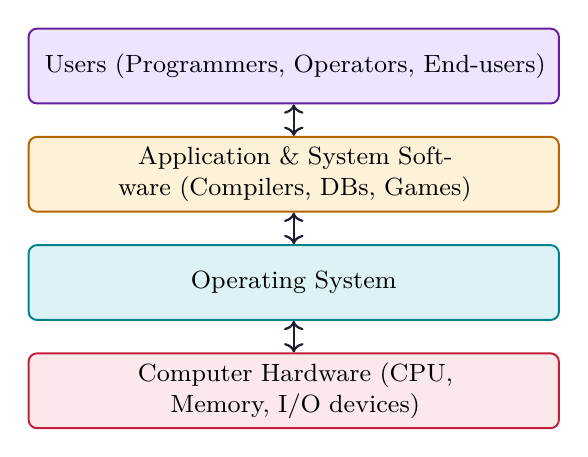
\begin{tikzpicture}[node distance=0.8cm, thick, font=\small]
  \node[block, text width=6.5cm, fill=hdrpurple, draw=mypurple] (users) {Users (Programmers, Operators, End-users)};
  \node[block, text width=6.5cm, fill=hdramber, draw=myamber, below=0.4cm of users] (apps) {Application \& System Software (Compilers, DBs, Games)};
  \node[block, text width=6.5cm, fill=hdrteal, draw=myteal, below=0.4cm of apps] (os) {Operating System};
  \node[block, text width=6.5cm, fill=hdrred, draw=myred, below=0.4cm of os] (hw) {Computer Hardware (CPU, Memory, I/O devices)};

  \draw[arrow, <->] (users) -- (apps);
  \draw[arrow, <->] (apps) -- (os);
  \draw[arrow, <->] (os) -- (hw);
\end{tikzpicture}
\end{tcolorbox}

\subsection{Core Functions of an Operating System}

\begin{tcolorbox}[defbox, title={\textbf{Definition: Operating System}}]
An \textbf{Operating System} is a system software that manages computer hardware, software resources, and provides common services for computer programs.
\end{tcolorbox}

From an engineering perspective, the functions of an OS can be classified into five major resource management categories:\par\noindent
\begin{tabularx}{\linewidth}{|B{3.2cm}|Y|}
\hline
\textbf{Function} & \textbf{\color{myteal}Description and Key Responsibilities} \\
\hline
\textbf{Process Management} & Creation, execution, scheduling, synchronization, and termination of active processes. \\
\hline
\textbf{Memory Management} & Tracking free and allocated memory spaces, page mapping, swapping, and virtual memory allocation. \\
\hline
\textbf{File System Management} & Organising directories, files, mapping files to secondary storage, and access controls. \\
\hline
\textbf{Device (I/O) Management} & Buffering, caching, spooling, device drivers, and disk head scheduling. \\
\hline
\textbf{Protection \& Security} & Controlling user access, authentication, preventing unauthorized access, and threat mitigation. \\
\hline
\end{tabularx}

% ===============================================================================
\section{Evolution of Operating Systems}
% ===============================================================================

Operating systems have evolved from simple manual job setups on mainframes to complex distributed real-time systems.

\subsection{Batch Processing Systems}
Early mainframes used a batch system where the user had no direct access to the machine. Jobs were prepared offline on punched cards and grouped into batches by an operator.
\begin{itemize}[leftmargin=*, itemsep=3pt]
  \item \textbf{Working Principle:} A program called the \textbf{resident monitor} stayed in memory, automatically loading and running subsequent jobs from the tape/card reader one after another.
  \item \textbf{Drawback:} No interactive user control, and extremely low CPU utilization due to the speed disparity between mechanical I/O devices (slow) and electronic CPU (fast).
\end{itemize}

\subsection{Interactive \& Multi-Programmed Systems}
To overcome batch limitations, multi-programmed systems kept multiple jobs in memory simultaneously. When one job had to wait for I/O, the OS switched CPU execution to another job.
\begin{itemize}[leftmargin=*, itemsep=3pt]
  \item \textbf{Interactive Systems:} Allowed direct communication between the user and system via a keyboard/terminal, giving immediate feedback.
\end{itemize}

\subsection{Time-Sharing Systems}
Time-sharing is a logical extension of multi-programming that provides fast interactive response times.
\begin{itemize}[leftmargin=*, itemsep=3pt]
  \item \textbf{Working Principle:} The CPU executes multiple jobs by switching among them extremely fast using a fixed time quantum (slice). Each user gets a dedicated, albeit small, fraction of the CPU time, giving the illusion of a dedicated machine.
  \item \textbf{Key Goal:} Minimizing \textbf{response time} for multiple simultaneous users.
\end{itemize}

% ===============================================================================
\section{Specialized Operating Systems}
% ===============================================================================

\subsection{Real-Time Systems (RTS)}
A \textbf{Real-Time Operating System (RTOS)} is used when rigid time requirements are placed on the operation of a processor or the flow of data. The correctness of an RTOS depends not only on the logical result of computation but also on the \textbf{time} at which it is delivered.

\begin{tcolorbox}[defbox, title={\textbf{Definition: Real-Time Systems}}]
A \textbf{Real-Time System} guarantees that critical tasks are completed within strict, specified time constraints (deadlines).
\end{tcolorbox}

Real-time systems are classified into two categories based on the severity of missing deadlines:\par\noindent
\begin{tabularx}{\linewidth}{|B{3.2cm}|Y|Y|}
\hline
\textbf{Feature} & \textbf{\color{myred}Hard Real-Time System} & \textbf{\color{myteal}Soft Real-Time System} \\
\hline
\textbf{Deadline Violation} & Catastrophic system failure. & Performance degradation only. \\
\hline
\textbf{Tolerance} & Zero tolerance. Deadlines must be met. & Occasional misses are tolerated. \\
\hline
\textbf{Memory Support} & Virtual memory is usually disabled. & Virtual memory is allowed. \\
\hline
\textbf{Examples} & pacemakers, missile guidance, airbags. & Video streaming, online gaming, audio. \\
\hline
\end{tabularx}

\subsection{Multi-Threading Systems}
A \textbf{thread} (or lightweight process) is a basic unit of CPU utilization. In a multi-threading operating system, a single process can spawn multiple concurrent threads of execution, all sharing the same code segment, data segment, and system resources, but having their own thread ID, program counter, register set, and stack.

\begin{itemize}[leftmargin=*, itemsep=3pt]
  \item \textbf{Benefits:} Responsiveness (non-blocking UI), resource sharing (threads share process memory), economy (context switching is faster than process creation), and multicore utilization.
\end{itemize}

\newpage
% ===============================================================================
% MANDATORY QUICK REVISION PAGE
% ===============================================================================
\begin{center}
  {\large\bfseries\color{myred} Quick Revision --- Module 1}\\[3pt]
  {\small\color{mydark} Introduction to Operating Systems $|$ OE-EC604B}
\end{center}
\noindent{\color{myred}\rule{\linewidth}{1.2pt}}
\vspace{4pt}

\begin{tcolorbox}[formulabox, title={\textbf{Key Evolution Properties at a Glance}}]
\renewcommand{\arraystretch}{1.3}
\begin{tabularx}{\linewidth}{B{3.8cm} X}
Batch OS & Low CPU utilization, high turnaround time, offline execution. \\[4pt]
Multiprogramming & High CPU utilization, keeps multiple jobs in memory, switches on I/O. \\[4pt]
Time-Sharing & Fixed time-slice (quantum), interactive, minimizes response time. \\[4pt]
Hard Real-Time & Strict deadlines, safety-critical, no virtual memory, predictable delay. \\[4pt]
Soft Real-Time & Best-effort deadlines, priority scheduling, virtual memory allowed.
\end{tabularx}
\end{tcolorbox}

\begin{tcolorbox}[defbox, title={\textbf{One-Line Definitions}}]
\begin{itemize}[leftmargin=*, itemsep=2.5pt, topsep=0pt]
  \item \textbf{Operating System:} System software managing hardware resources and acting as a user-hardware interface.
  \item \textbf{Spooling:} Simultaneous Peripheral Operations On-Line; placing I/O data in disk buffer to speed up batch execution.
  \item \textbf{Multiprogramming:} OS technique running multiple jobs concurrently to maximize CPU utilization.
  \item \textbf{Time-Sharing:} Preemptive multiprogramming where CPU switches quickly between users using a time slice.
  \item \textbf{Real-Time OS:} Time-bound operating system designed for deterministic response times and deadlines.
  \item \textbf{Hard Real-Time:} OS where missing a single task deadline results in catastrophic system failure.
  \item \textbf{Soft Real-Time:} OS where deadlines are preferred but occasional misses do not cause system failure.
  \item \textbf{Thread:} A lightweight process representing a single sequential flow of control within a process.
  \item \textbf{Resident Monitor:} Early batch supervisor program residing in memory to load jobs automatically.
\end{itemize}
\end{tcolorbox}

\begin{tcolorbox}[exambox, title={\textbf{Frequently Asked / Viva Questions}}]
\begin{enumerate}[topsep=0pt, label=\textbf{Q\arabic*.}, itemsep=5pt]
  \item \Q{What are the primary objectives of an operating system?}
    To make the computer system convenient to use for the user, and to allocate and manage the hardware resources (CPU, memory, devices) in an efficient and fair manner.
  \item \Q{Explain the difference between Multiprogramming and Multiprocessing.}
    Multiprogramming keeps multiple processes in main memory simultaneously on a single CPU, switching between them to keep the CPU busy. Multiprocessing involves a computer system with two or more physical CPUs executing processes in parallel.
  \item \Q{What is spooling? How does it differ from buffering?}
    Spooling uses the disk as a large buffer to store incoming/outgoing jobs and data for slow peripheral devices (like printers), enabling concurrent CPU processing. Buffering is a temporary storage area in main memory used during I/O transfers to smooth out speed differences.
  \item \Q{Differentiate between Hard Real-Time and Soft Real-Time systems.}
    Hard Real-Time systems have strict, non-negotiable deadlines where any failure causes catastrophic system collapse (e.g., flight controller). Soft Real-Time systems treat deadlines as highly desirable but tolerate occasional misses without failure (e.g., video player).
  \item \Q{What is the time-sharing concept? Which scheduling is typically used?}
    Time-sharing allows multiple users to share a single CPU interactively. The OS allocates a small time slice (quantum) to each user process and switches preemptively using Round Robin scheduling to maintain low response times.
  \item \Q{List the primary resource management functions of an OS.}
    Process management, Memory management, File system management, I/O device management, and Protection/Security management.
  \item \Q{Why is virtual memory usually not supported in hard real-time systems?}
    Virtual memory introduces unpredictable time delays due to page faults and disk access latency, which violates the strict deterministic timing requirements of hard real-time systems.
  \item \Q{Explain how multithreading improves application responsiveness.}
    By splitting execution into multiple threads, an application can execute background tasks (like disk writing or computations) in one thread while the main thread keeps responding to user actions (like button clicks) without freezing the UI.
  \item \Q{What is the role of a resident monitor in early batch systems?}
    It was the first operating program. It resided in main memory and automatically handled job transitions by reading the next job card/tape as soon as the current one finished, reducing setup time.
  \item \Q{Why is CPU scheduling required in multiprogrammed systems?}
    When the active process performs I/O, it must wait. To prevent the CPU from sitting idle, CPU scheduling selects another ready process from memory to execute, maximizing CPU utilization.
\end{enumerate}
\end{tcolorbox}

\begin{tcolorbox}[tikzbox, title={Comparative Analysis of Operating Systems}]
\renewcommand{\arraystretch}{1.4}
\par\noindent
\begin{tabularx}{\linewidth}{|B{2.2cm}|>{\small\centering\arraybackslash}X|>{\small\centering\arraybackslash}X|>{\small\centering\arraybackslash}X|}
\hline
\textbf{System Type} & \textbf{\color{myred}Primary Goal} & \textbf{\color{myteal}CPU Utilization} & \textbf{\color{myamber}Interaction Level} \\
\hline
\textbf{Batch} & Maximize Throughput & Low to Moderate & None (offline jobs) \\
\hline
\textbf{Multiprogrammed} & Maximize CPU usage & High (context switches on I/O) & Low (background jobs) \\
\hline
\textbf{Time-Sharing} & Minimize Response Time & Moderate to High & Very High (interactive) \\
\hline
\textbf{Real-Time} & Guarantee Deadline & Secondary concern & Low (automated control) \\
\hline
\end{tabularx}
\end{tcolorbox}

\end{document}
